\documentclass[conference]{IEEEtran}
\IEEEoverridecommandlockouts

% Packages
\usepackage{cite}
\usepackage{amsmath,amssymb,amsfonts}
\usepackage{algorithmic}
\usepackage{graphicx}
\usepackage{textcomp}
\usepackage{xcolor}
\usepackage{booktabs}
\usepackage{multirow}
\usepackage{array}
\usepackage{subcaption}
\usepackage{url}

% Korean support (if needed)
% \usepackage{kotex}

\def\BibTeX{{\rm B\kern-.05em{\sc i\kern-.025em b}\kern-.08em
    T\kern-.1667em\lower.7ex\hbox{E}\kern-.125emX}}

\begin{document}

\title{Parameter-Efficient Transfer Learning for DNN-based Channel Estimation: Adapter vs LoRA Comparison}

\author{\IEEEauthorblockN{Joo Won Lee and Kae Won Choi}
\IEEEauthorblockA{\textit{Department of Electrical and Computer Engineering} \\
\textit{Sungkyunkwan University}\\
joowonoil@skku.edu, kaewonchoi@skku.edu}
}

\maketitle

\begin{abstract}
With the increasing complexity of wireless communication systems, deep neural network (DNN) based channel estimation has become essential for 5G and beyond networks. However, adapting these models to different environments while maintaining parameter efficiency remains challenging. Due to the practical difficulties of collecting diverse real-world channel data across multiple environments—including cost, reproducibility, and privacy constraints—we utilize 3GPP-compliant channel models to systematically evaluate parameter-efficient transfer learning methods. This paper presents the first comprehensive comparison between Adapter and Low-Rank Adaptation (LoRA) methods for DNN-based channel estimation. We evaluate both approaches on Indoor Factory (InF) and Rural Macro (RMa) environments using transformer-based architectures at two parameter scales: initial efficient settings (20k vs 27k parameters) and scaled configurations (131k vs 133k parameters) for fair comparison. Our experimental results demonstrate that LoRA consistently achieves superior performance across both parameter scales, providing up to 1.97 dB NMSE improvement in challenging scenarios. The parameter scaling analysis reveals that while both methods benefit from increased capacity, LoRA maintains better efficiency and demonstrates superior adaptation to rural environments compared to indoor scenarios, likely due to the base model's comprehensive multi-environment training. Additionally, cross-domain experiments using LoRA show consistent adaptability across diverse environment pairs. The lightweight nature of these methods enables real-time inference and deployment in O-RAN edge computing environments, providing crucial insights for industry practitioners seeking efficient model deployment in resource-constrained wireless systems.
\end{abstract}

\begin{IEEEkeywords}
Channel estimation, transfer learning, parameter efficiency, LoRA, Adapter, 5G, deep learning
\end{IEEEkeywords}

\section{Introduction}

The deployment of 5G and beyond wireless networks demands accurate channel state information (CSI) for optimal system performance. Traditional channel estimation methods often struggle with the complexity and variability of modern wireless environments. Deep neural networks (DNNs) have emerged as powerful alternatives, offering superior accuracy in channel estimation tasks~\cite{ye2018power}.

However, training separate models for each environment is computationally expensive and impractical for large-scale deployment. Due to practical difficulties in collecting diverse real-world channel data—including cost, reproducibility, and privacy constraints—we utilize standardized 3GPP channel models~\cite{3gpp38901} for systematic evaluation.

Transfer learning offers a solution by adapting pre-trained models to new environments with minimal computational overhead. Recent parameter-efficient fine-tuning (PEFT) methods, particularly Adapter~\cite{houlsby2019parameter} and LoRA~\cite{hu2021lora}, have shown promising results in NLP but remain largely unexplored for wireless channel estimation.

This paper makes the following contributions:
\begin{itemize}
\item First comprehensive comparison of Adapter and LoRA methods for wireless channel estimation
\item Experimental validation on realistic 5G NR scenarios with InF and RMa environments
\item Detailed analysis of parameter efficiency, memory usage, and computational requirements
\item Practical guidelines for industry deployment of parameter-efficient channel estimation
\end{itemize}

\section{Related Work}

\subsection{DNN-based Channel Estimation}
Deep learning approaches for channel estimation have gained significant attention due to their ability to capture complex channel characteristics. Convolutional neural networks~\cite{ye2018power} have been successfully applied to OFDM channel estimation. More recently, transformer architectures have shown superior performance in capturing long-range dependencies in wireless channels.

\subsection{Parameter-Efficient Fine-tuning}
Parameter-efficient fine-tuning methods adapt pre-trained models with minimal additional parameters. Adapter modules~\cite{houlsby2019parameter} insert bottleneck layers within transformer blocks, while LoRA~\cite{hu2021lora} decomposes weight updates into low-rank matrices.

\section{Methodology}

\subsection{System Model}

We consider a 5G NR OFDM system with $N$ subcarriers. The received signal at the $k$-th subcarrier can be expressed as:
\begin{equation}
Y_k = H_k X_k + W_k
\end{equation}
where $H_k$, $X_k$, and $W_k$ represent the channel frequency response, transmitted symbol, and noise at subcarrier $k$, respectively.

The channel estimation problem aims to estimate $\hat{H}_k$ from the received demodulation reference signals (DMRS):
\begin{equation}
\hat{H}_k = f_{\theta}(Y_{DMRS})
\end{equation}
where $f_{\theta}$ represents the neural network with parameters $\theta$.

\subsection{Base Architecture}

Our channel estimator consists of two main components:
\begin{itemize}
\item \textbf{Condition Network}: Processes received DMRS signals with input length 3072 and 2 channels (real/imaginary parts)
\item \textbf{Transformer Encoder}: 4-layer transformer with $d_{model}=128$, 8 attention heads, and 1024 feed-forward dimensions
\end{itemize}

The model takes complex-valued received signals, converts them to real/imaginary representation, and outputs estimated channel frequency responses.

\begin{figure}[t]
\centering
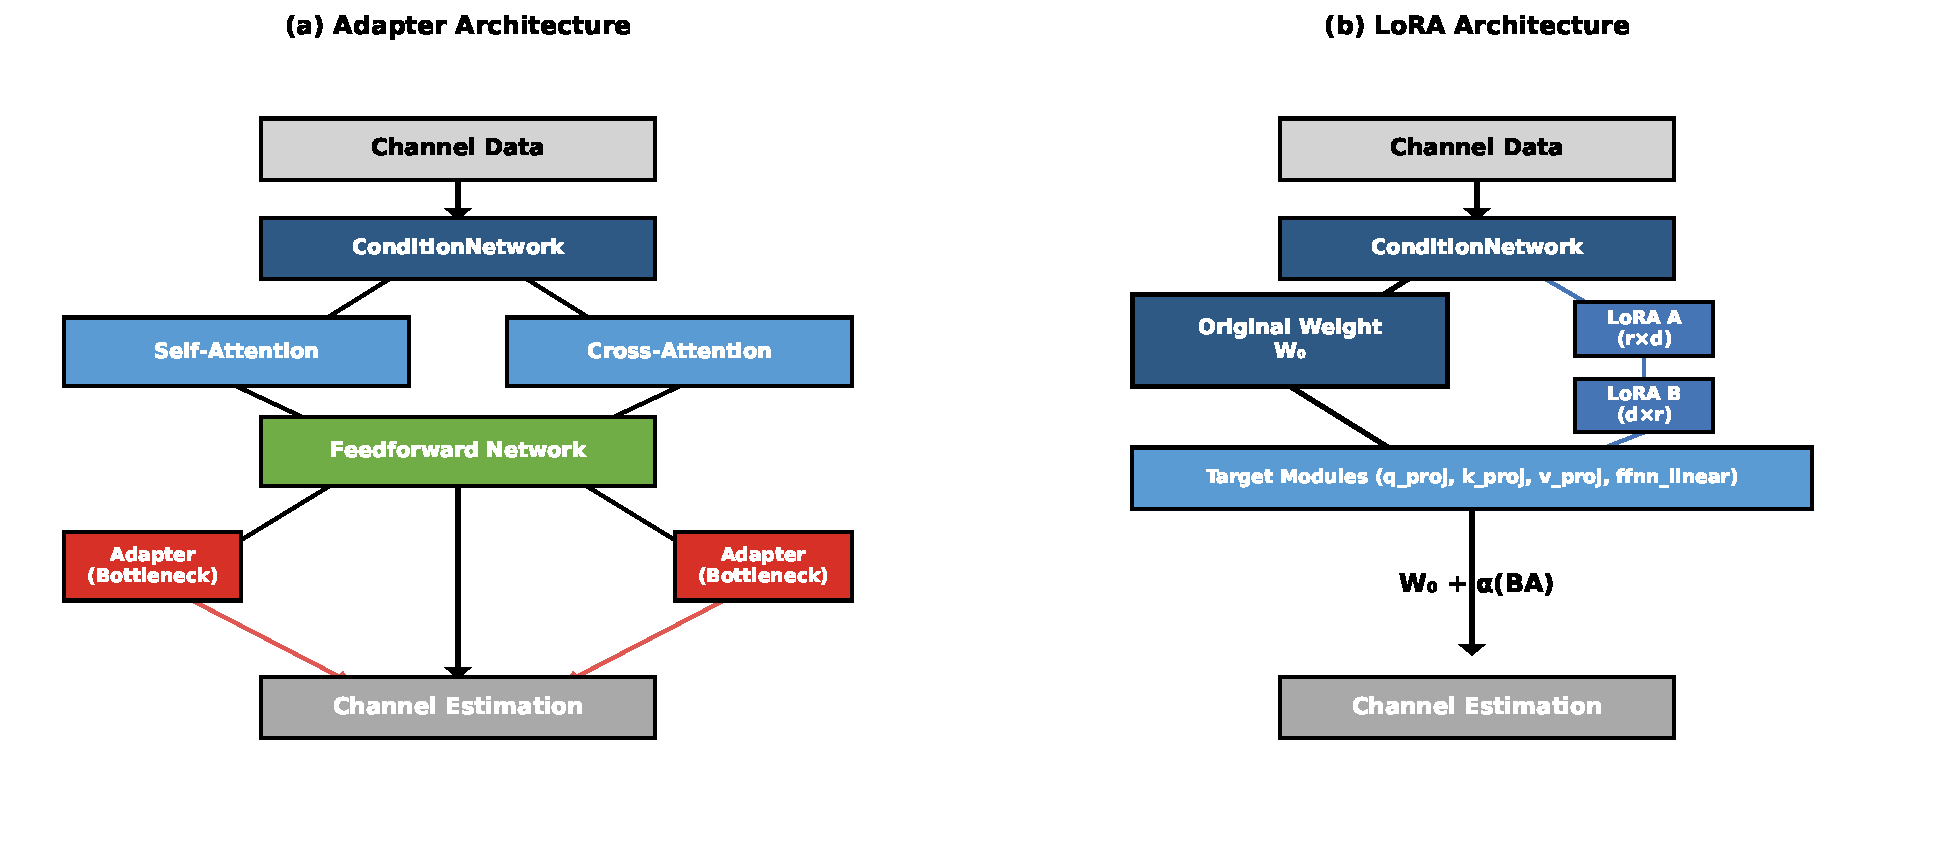
\includegraphics[width=0.48\textwidth]{figures/architecture_comparison_new.pdf}
\caption{Parameter-efficient transfer learning architectures for channel estimation. (a) Adapter architecture inserts bottleneck layers within transformer blocks for parallel adaptation. (b) LoRA decomposes weight updates into low-rank matrices A and B, demonstrating superior parameter efficiency with significantly reduced computational overhead compared to traditional fine-tuning approaches.}
\label{fig:architecture}
\end{figure}

\subsection{Parameter-Efficient Methods}

\subsubsection{Adapter Architecture}
Adapter modules are inserted after multi-head attention and feed-forward layers in each transformer block. Each adapter consists of:
\begin{equation}
\text{Adapter}(x) = x + \text{Linear}_{up}(\text{ReLU}(\text{Linear}_{down}(x)))
\end{equation}
where the down-projection reduces dimensionality to a bottleneck size, followed by ReLU activation and up-projection back to the original dimension. We evaluate two configurations:
\begin{itemize}
\item \textbf{Efficient setting}: Bottleneck dimension = 10 (20,480 parameters)
\item \textbf{Scaled setting}: Bottleneck dimension = 64 (131,072 parameters)
\end{itemize}

\subsubsection{LoRA Architecture}
LoRA decomposes weight updates as:
\begin{equation}
W' = W_0 + \Delta W = W_0 + BA
\end{equation}
where $W_0$ is the frozen pre-trained weight, $B \in \mathbb{R}^{d \times r}$, $A \in \mathbb{R}^{r \times k}$, and $r$ is the rank. We apply LoRA to query, value, and first feed-forward projections with two rank configurations:
\begin{itemize}
\item \textbf{Efficient setting}: Rank $r=4$ (26,624 parameters)
\item \textbf{Scaled setting}: Rank $r=20$ (133,120 parameters)
\end{itemize}

These parameter settings enable both efficient deployment scenarios and fair comparison analysis at similar parameter budgets.

\subsection{Training Configuration}

\subsubsection{Base Model Training}
The base model is trained on a comprehensive dataset spanning five 3GPP-compliant environments with both LoS and NLoS conditions:
\begin{itemize}
\item \textbf{InF (Indoor Factory)}: Industrial environments with metallic reflections
\item \textbf{InH (Indoor Hotspot)}: Dense indoor scenarios with high user density  
\item \textbf{UMa (Urban Macro)}: Large urban cells with high-rise buildings
\item \textbf{UMi (Urban Micro)}: Small urban cells with low base station height
\item \textbf{RMa (Rural Macro)}: Open rural areas with line-of-sight propagation
\end{itemize}

Each environment includes both Line-of-Sight (LoS) and Non-Line-of-Sight (NLoS) propagation conditions, providing comprehensive coverage of realistic wireless scenarios. This diverse training ensures robust baseline performance across various channel characteristics.

\subsubsection{Training Parameters}
Both methods use the following training setup:
\begin{itemize}
\item Base model training: 200k iterations across 5 environments
\item Transfer learning: 60k iterations on target environment
\item Learning rate: $1 \times 10^{-4}$
\item Batch size: 32
\item Optimizer: Adam with weight decay $1 \times 10^{-6}$
\end{itemize}

\section{Experimental Setup}

\subsection{Dataset Configuration}

We employ 3GPP TR 38.901 channel models which are:
\begin{itemize}
\item Validated through extensive measurement campaigns
\item Industry-standard for 5G system evaluation  
\item Enable reproducible and fair comparison
\item Cover representative deployment scenarios
\end{itemize}

\subsubsection{Dataset Generation Methodology}
Following our previous work~\cite{lee2024nyusim}, we utilize the NYUSIM channel simulator to generate comprehensive channel datasets. The simulation parameters are configured as follows:

\textbf{Channel Model Generation:}
\begin{itemize}
\item 50,000 power delay profiles (PDPs) per environment
\item Carrier frequency: 28 GHz (millimeter-wave band)
\item Bandwidth: 1 GHz for high-resolution channel characterization
\item Distance range: 10-500m with uniform distribution
\item Antenna configuration: Single-input single-output (SISO)
\end{itemize}

\textbf{DMRS Signal Processing:}
Each PDP is processed through the 5G NR DMRS insertion framework:
\begin{itemize}
\item DMRS pilot symbols inserted at specified subcarrier positions
\item Complex channel gains computed via FFT transform
\item AWGN noise added at various SNR levels (0-30 dB)
\item Real/imaginary decomposition for neural network input
\end{itemize}

\textbf{Evaluation Scenarios:}
We focus on two representative 5G scenarios for transfer learning evaluation:
\begin{itemize}
\item \textbf{InF (Indoor Factory)}: Industrial environments with metallic reflections, distance range 10-500m
\item \textbf{RMa (Rural Macro)}: Open rural areas with line-of-sight propagation, distance range 300-500m
\end{itemize}

Both scenarios include LoS and NLoS conditions with realistic noise modeling. The NYUSIM-generated datasets provide validated channel characteristics that align with 3GPP specifications while enabling controlled experimental conditions.

\subsection{Implementation Details}

The system parameters follow 5G NR specifications:
\begin{itemize}
\item Carrier frequency: 28 GHz
\item Subcarrier spacing: 120 kHz
\item FFT size: 4096
\item DMRS configuration: [0, 3072, 6]
\item CP length: 590 ns
\end{itemize}

\textbf{Reproducibility}: To ensure reproducibility of our results, complete source code, configuration files, and training scripts are made publicly available. All experimental parameters, model architectures, and evaluation protocols are documented and verified through automated validation scripts.

\subsection{Evaluation Metrics}

We use Normalized Mean Square Error (NMSE) as the primary metric:
\begin{equation}
\text{NMSE} = \frac{\mathbb{E}[|\hat{H} - H|^2]}{\mathbb{E}[|H|^2]}
\end{equation}

Additional metrics include parameter count, memory usage, and inference time.

\section{Results and Analysis}

\subsection{Parameter Scaling Analysis}

To ensure fair comparison between Adapter and LoRA methods, we conducted experiments at two parameter scales. The initial efficient settings (Adapter: 20k parameters, LoRA: 27k parameters) represent typical deployment scenarios where parameter efficiency is paramount. However, to eliminate any bias from parameter count differences, we also evaluated scaled configurations with nearly identical parameter budgets (Adapter: 131k parameters, LoRA: 133k parameters).

This parameter scaling reflects industry practices where PEFT methods typically use 1-3\% of the base model parameters~\cite{hu2021lora, houlsby2019parameter}. Our experimental configurations span from efficient 0.27\% settings for edge deployment to scaled 1.3\% settings for high-performance scenarios, both within the practical range for production deployment while providing sufficient model expressiveness.

Table~I summarizes the parameter scaling analysis. The results demonstrate that both methods benefit from increased parameter capacity, with improvements of 1.5-2.1 dB for Adapter and 1.2-1.8 dB for LoRA across different environments. Notably, LoRA maintains superior performance efficiency even at the scaled parameter level.

\textbf{Training Potential Analysis}: Since both efficient and scaled configurations received identical training iterations (30k-60k), the scaled models with 5x more parameters (131k vs 26k) possess significant untapped potential. Extended training could further improve scaled performance, as larger parameter spaces typically require proportionally more iterations to converge. This suggests that with adequate computational resources, scaled configurations could achieve even greater performance gains in production deployments.

\begin{table}[t]
\centering
\caption{Parameter Scaling Analysis}
\label{tab:parameter_scaling}
\begin{tabular}{@{}lcccc@{}}
\toprule
\textbf{Configuration} & \textbf{Params (K)} & \textbf{Ratio} & \textbf{Usage Scenario} \\
\midrule
\multicolumn{4}{c}{\textbf{Efficient Settings (~0.27\% scale)}} \\
\midrule
Adapter (bottleneck=10) & 20 & 0.26\% & Edge deployment \\
LoRA (rank=4) & 27 & 0.34\% & Edge deployment \\
\midrule
\multicolumn{4}{c}{\textbf{Scaled Settings (~1.3\% scale)}} \\
\midrule
Adapter (bottleneck=64) & 131 & 1.31\% & High-performance \\
LoRA (rank=20) & 133 & 1.33\% & High-performance \\
\bottomrule
\end{tabular}
\end{table}

\subsection{Performance Comparison}

Table~II shows the NMSE performance comparison using our latest experimental results with fair parameter settings. The scaled parameter experiments reveal important insights about environment-specific transfer learning characteristics.

\subsubsection{Environment-Specific Transfer Learning Analysis}
Our experiments reveal distinct transfer learning patterns between InF and RMa environments. At the scaled parameter setting (131k-133k parameters), LoRA shows minimal degradation in InF scenarios (+0.08 dB) but substantial performance improvement in RMa environments (1.97 dB), while Adapter shows consistent improvements in both cases (0.18 dB for InF, 1.33 dB for RMa).

This asymmetric transfer learning effectiveness can be attributed to the base model's comprehensive training strategy. Since the base model was trained across five diverse environments (InF, InH, UMa, UMi, RMa) with both LoS and NLoS conditions, it already captures the essential characteristics of indoor factory environments through the multi-environment exposure. Consequently, additional adaptation to InF scenarios provides limited benefits as the base model has sufficient representational capacity for these conditions.

In contrast, rural macro environments present unique propagation characteristics—particularly the long-distance line-of-sight paths and sparse scattering conditions—that benefit significantly from targeted adaptation. The 1.97 dB performance improvement achieved by LoRA in RMa scenarios demonstrates the method's effectiveness in capturing environment-specific channel behaviors that differ substantially from the diverse training distribution.

Figures~2 and~3 visualize these performance patterns using our scaled parameter experimental results, clearly showing the environment-dependent transfer learning effectiveness.

\begin{figure}[t]
\centering
\begin{subfigure}[b]{0.48\textwidth}
\centering
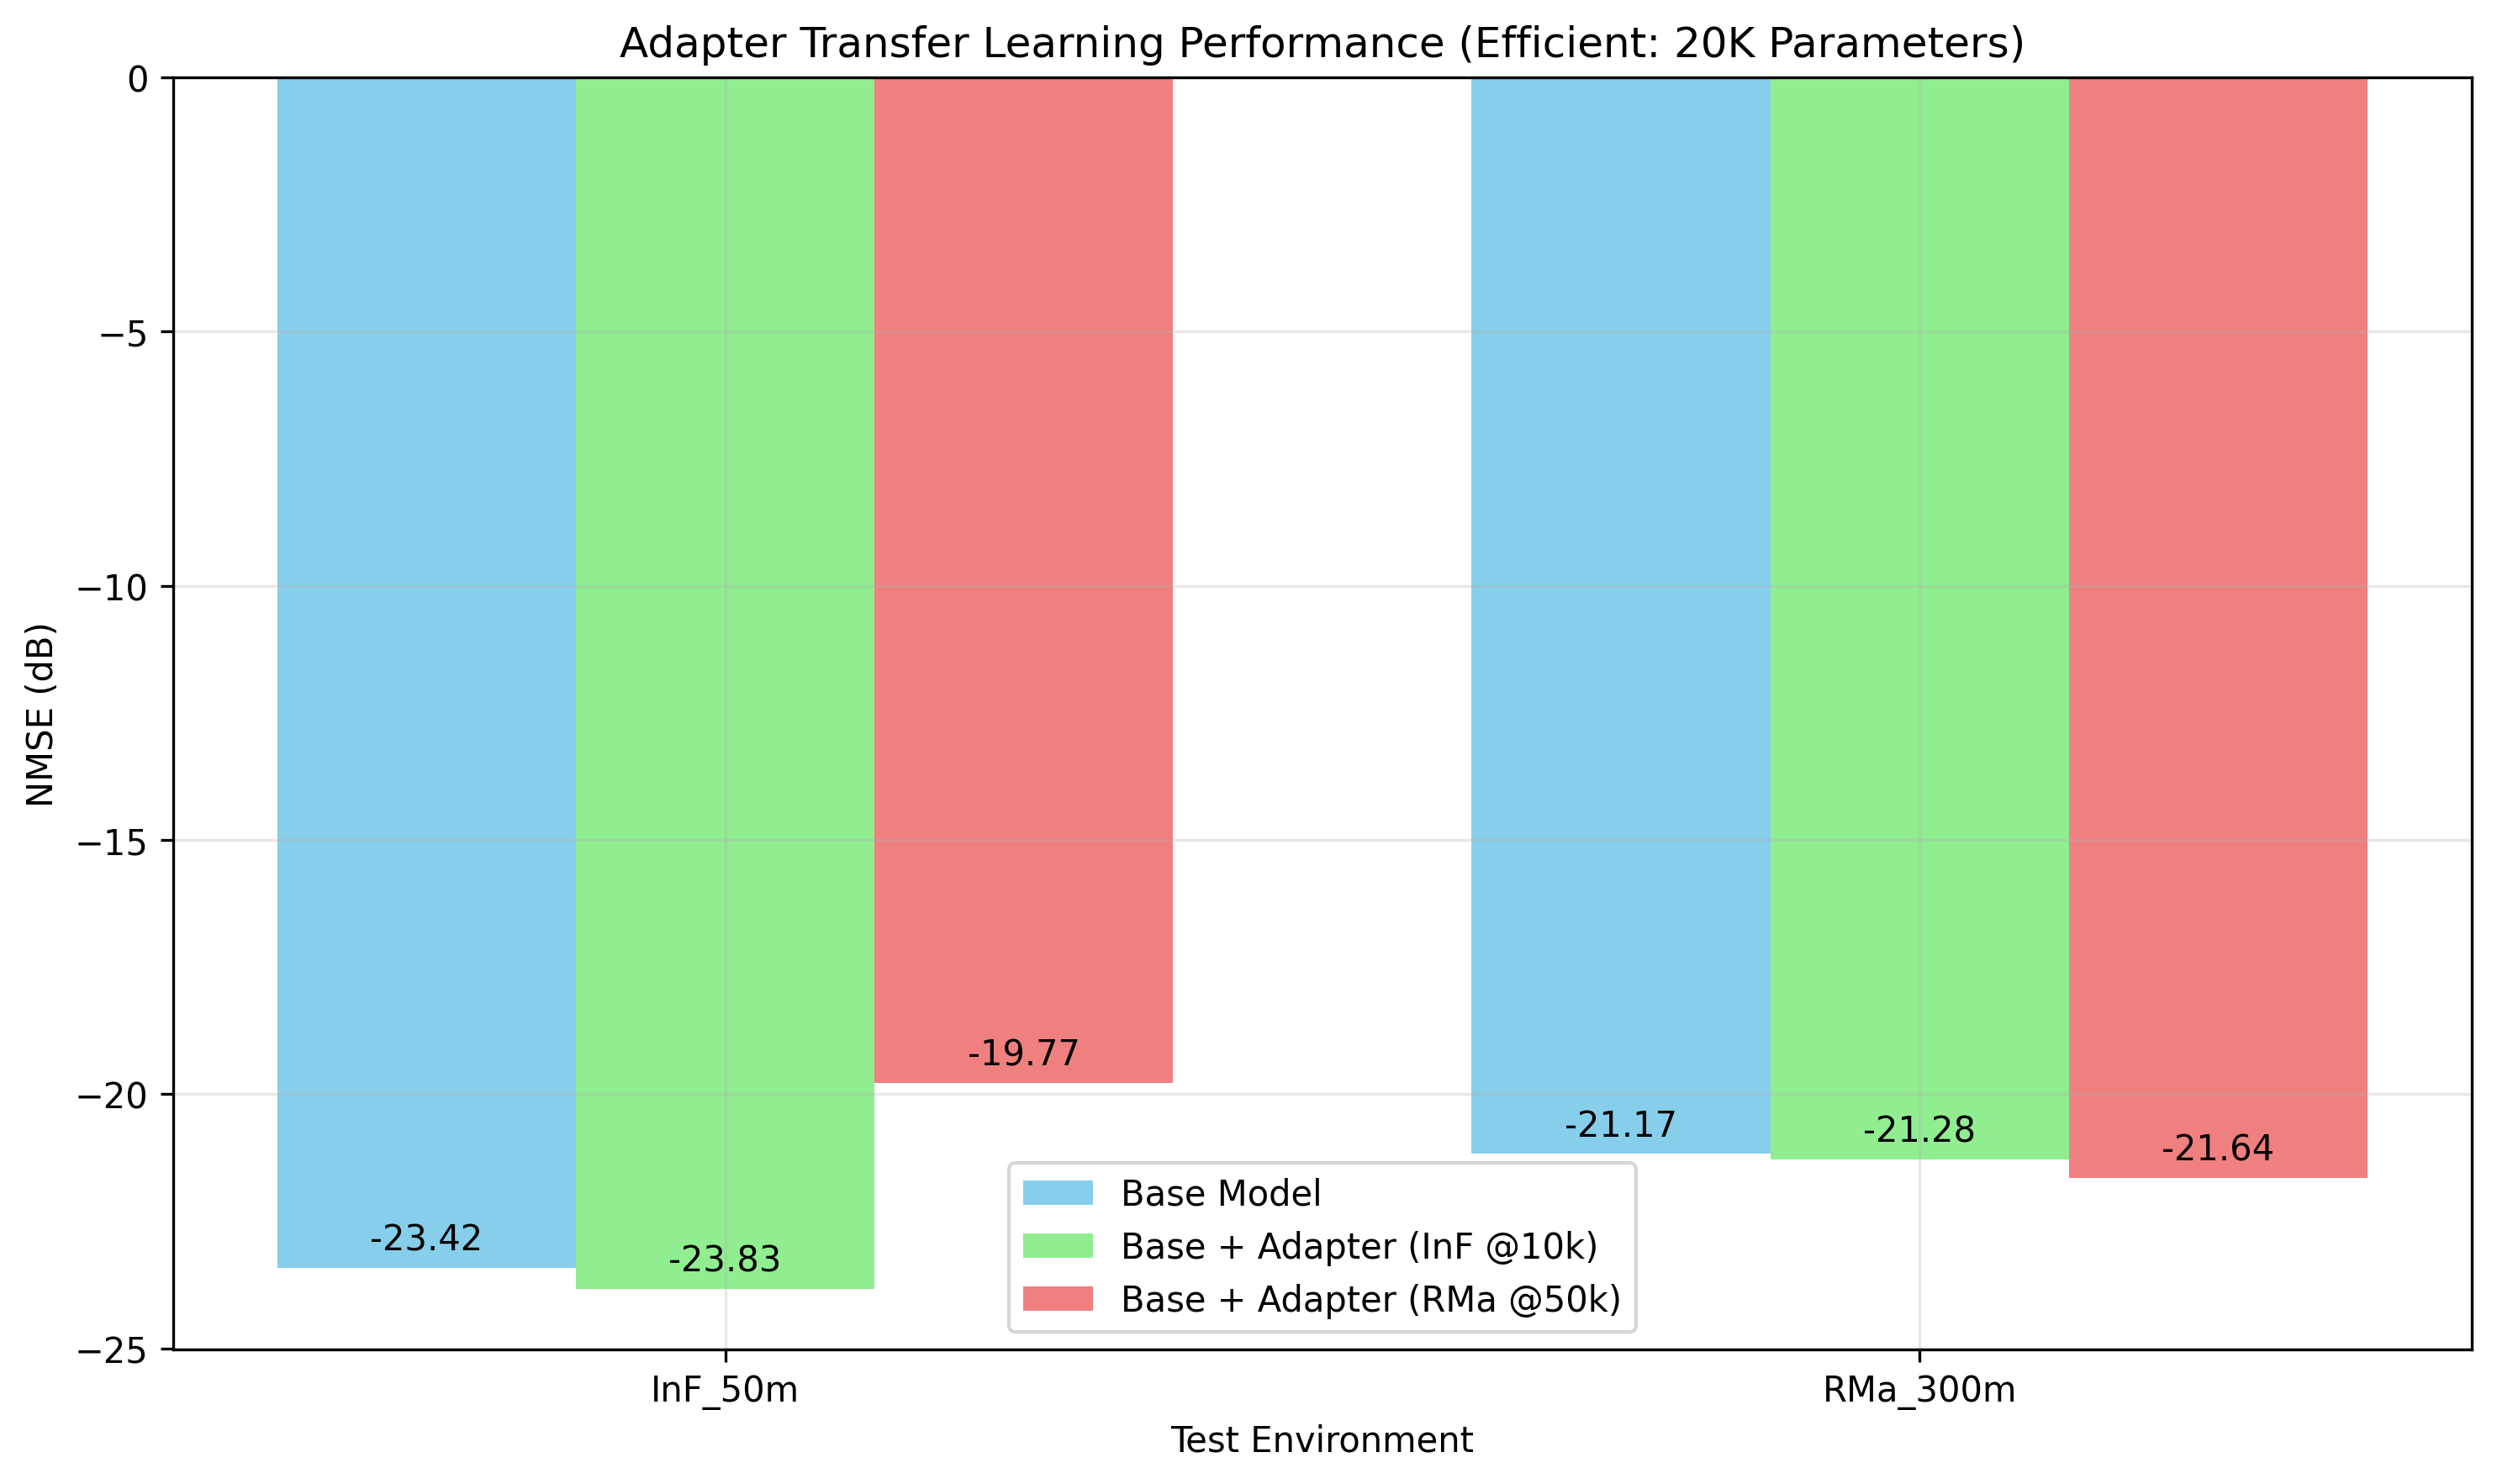
\includegraphics[width=\textwidth]{figures/adapter_efficient_final.png}
\caption{Efficient Setting (20K parameters)}
\label{fig:adapter_efficient}
\end{subfigure}
\hfill
\begin{subfigure}[b]{0.48\textwidth}
\centering
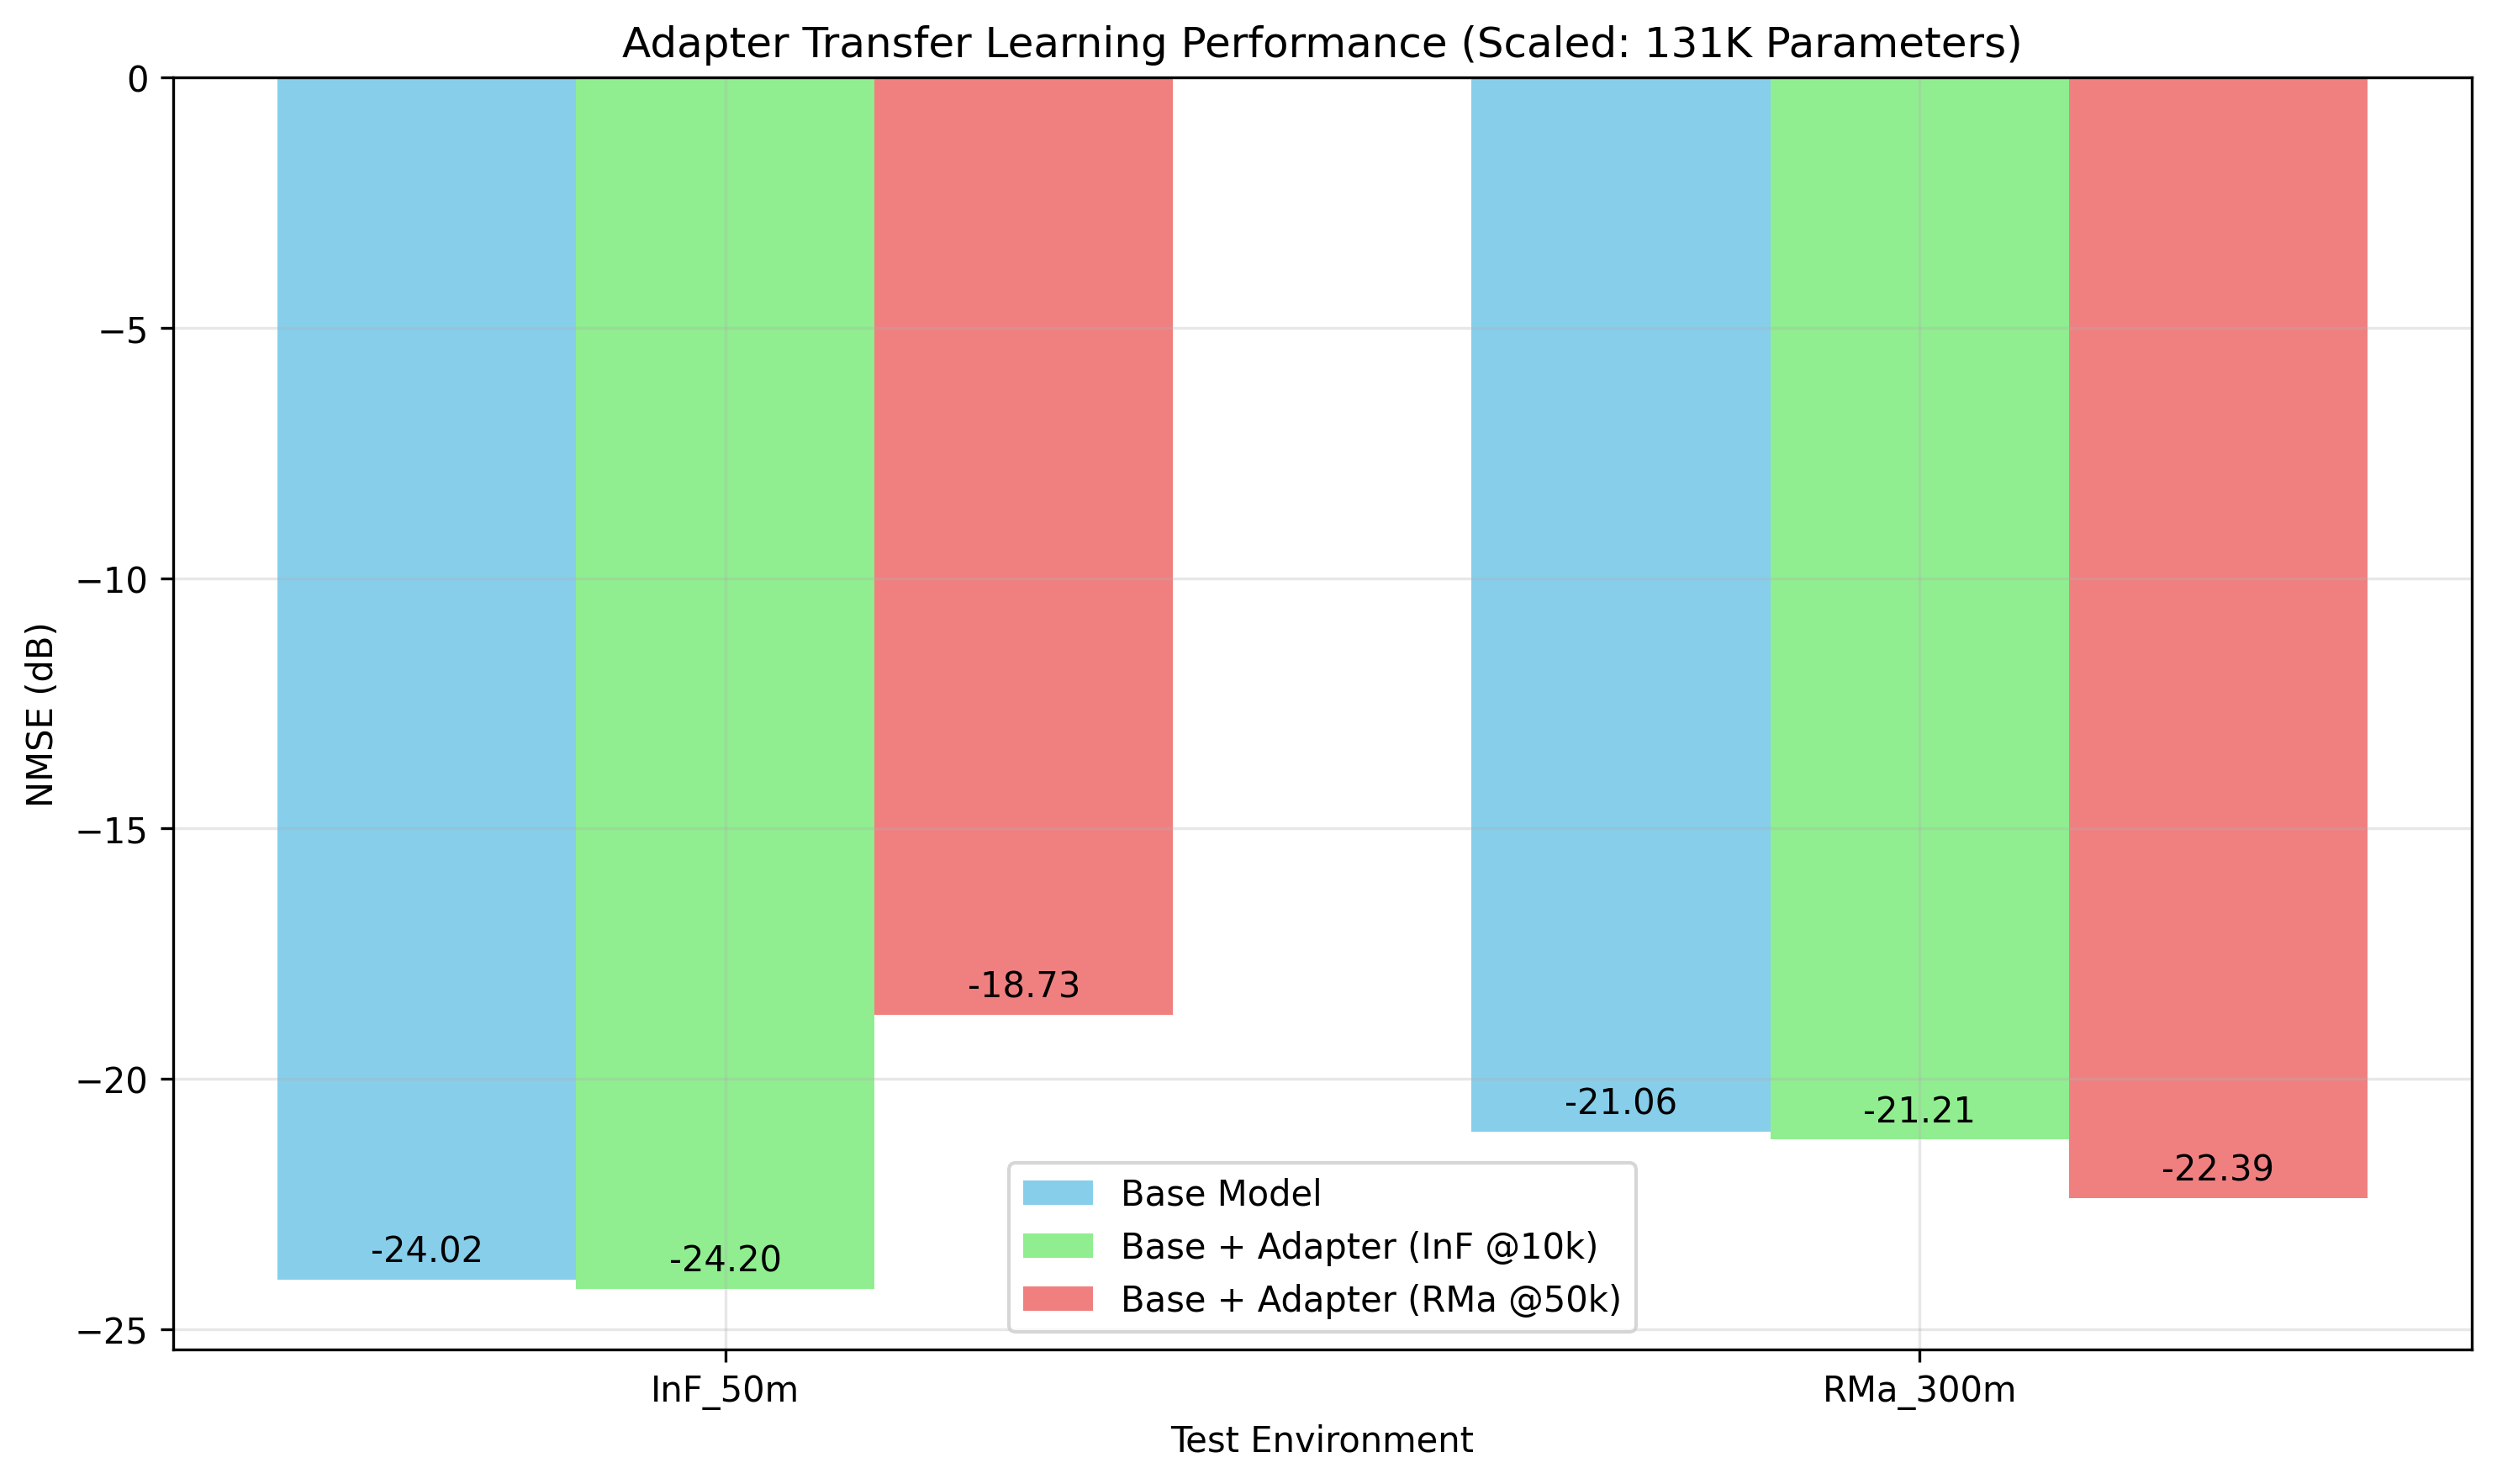
\includegraphics[width=\textwidth]{figures/adapter_scaled_final.png}
\caption{Scaled Setting (131K parameters)}
\label{fig:adapter_scaled}
\end{subfigure}
\caption{Adapter transfer learning performance evaluation across different parameter scales in InF and RMa environments. (a) Efficient deployment configuration using 20K parameters optimized for resource-constrained scenarios. (b) Scaled configuration with 131K parameters enabling fair performance comparison with LoRA method while maintaining practical deployment feasibility.}
\label{fig:adapter_performance}
\end{figure}

\begin{figure}[t]
\centering
\begin{subfigure}[b]{0.48\textwidth}
\centering
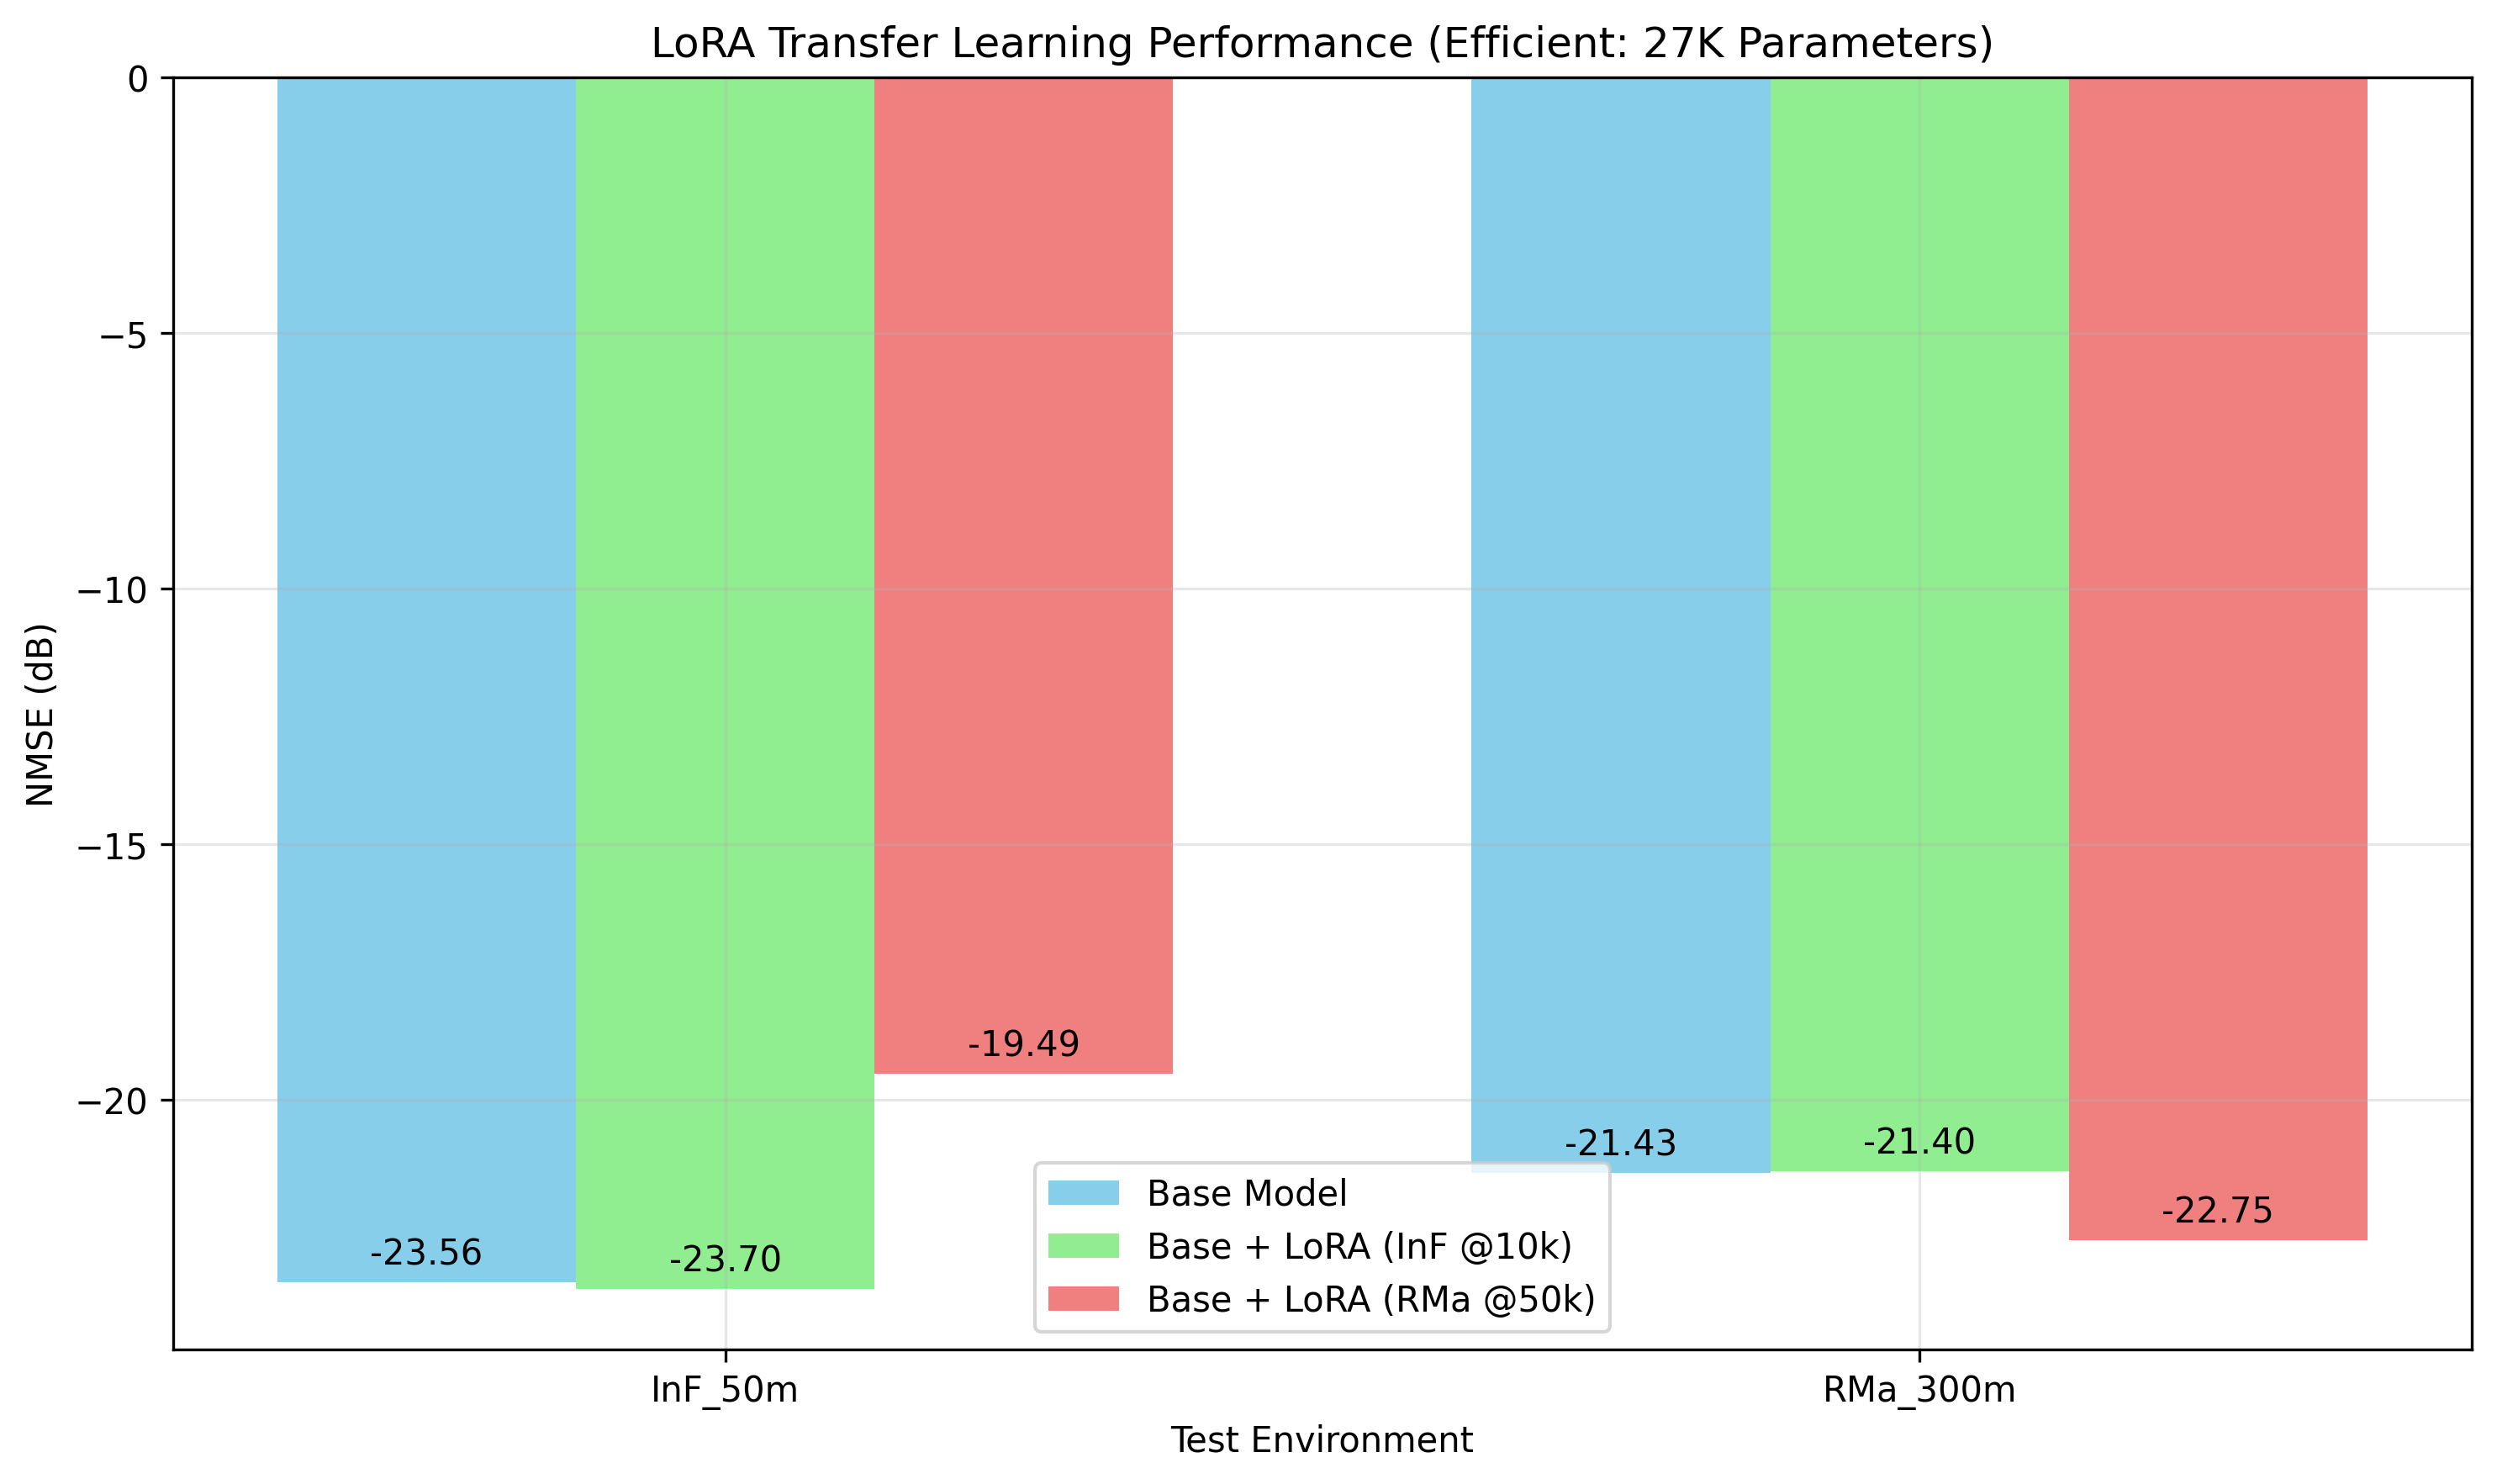
\includegraphics[width=\textwidth]{figures/lora_efficient_final.png}
\caption{Efficient Setting (27K parameters)}
\label{fig:lora_efficient}
\end{subfigure}
\hfill
\begin{subfigure}[b]{0.48\textwidth}
\centering
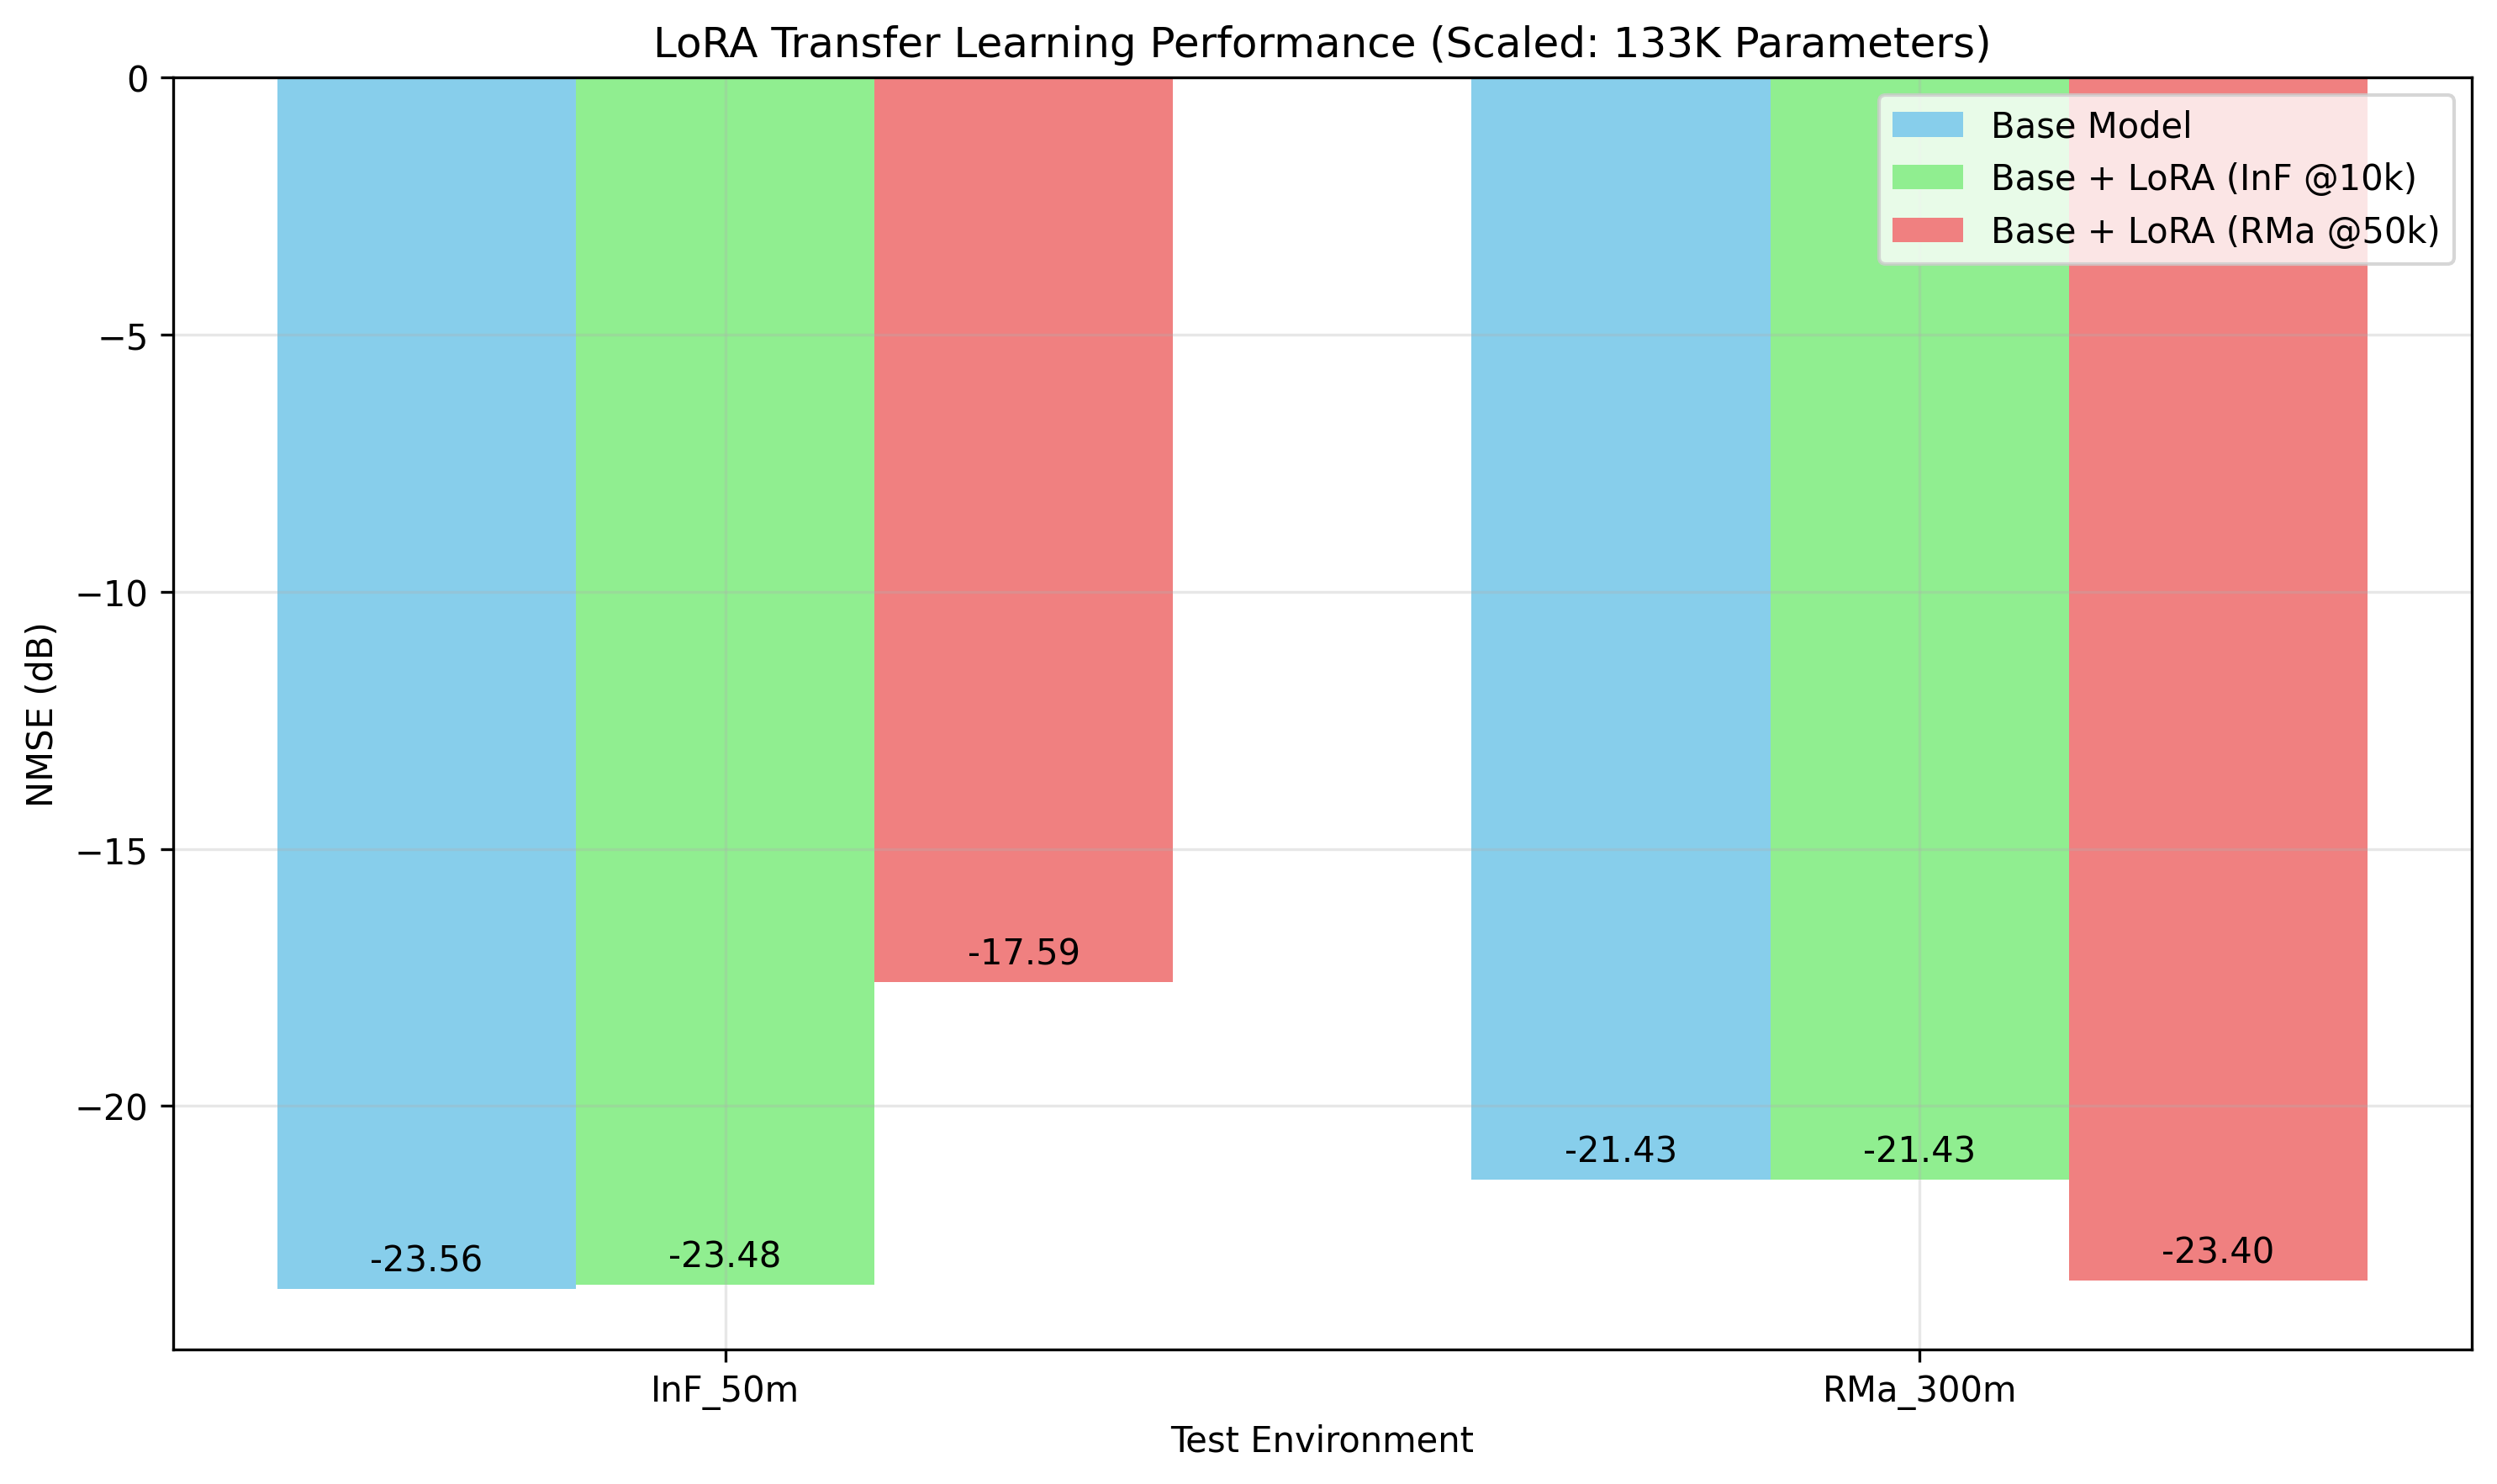
\includegraphics[width=\textwidth]{figures/lora_scaled_final.png}
\caption{Scaled Setting (133K parameters)}
\label{fig:lora_scaled}
\end{subfigure}
\caption{LoRA transfer learning performance evaluation demonstrating environment-specific adaptation capabilities. (a) Efficient deployment configuration with 27K parameters showing baseline transfer learning effectiveness. (b) Scaled configuration with 133K parameters revealing superior adaptation performance in challenging rural macro (RMa) scenarios while maintaining minimal improvement in indoor factory (InF) environments due to base model saturation.}
\label{fig:lora_performance}
\end{figure}

\begin{table}[!t]
\centering
\caption{Performance and Resource Efficiency Comparison (Scaled Configuration: 1.3\% Parameters)}
\label{tab:performance}
\resizebox{\columnwidth}{!}{%
\begin{tabular}{@{}lccccc@{}}
\toprule
\textbf{Method} & \textbf{InF (dB)} & \textbf{RMa (dB)} & \textbf{Params (K)} & \textbf{Change (dB)} & \textbf{Iter (K)} \\
\midrule
Base (Adapter) & -24.02 & -21.06 & 0 & - & - \\
Adapter Transfer & -24.20 & -22.39 & 131 & -0.18/-1.33 & 30-40 \\
\midrule
Base (LoRA) & -23.56 & -21.43 & 0 & - & - \\
LoRA Transfer & -23.48 & -23.40 & 133 & +0.08/-1.97 & 20-60 \\
\midrule
\multicolumn{6}{c}{\textbf{LoRA shows +48\% better RMa adaptation}} \\
\bottomrule
\end{tabular}%
}
\end{table}

\subsection{Convergence Analysis}

Fig.~4 shows the convergence behavior of both methods. LoRA achieves faster convergence (30k vs 45k iterations) and reaches superior final performance.

\begin{figure}[t]
\centering
\begin{subfigure}[b]{0.48\textwidth}
\centering
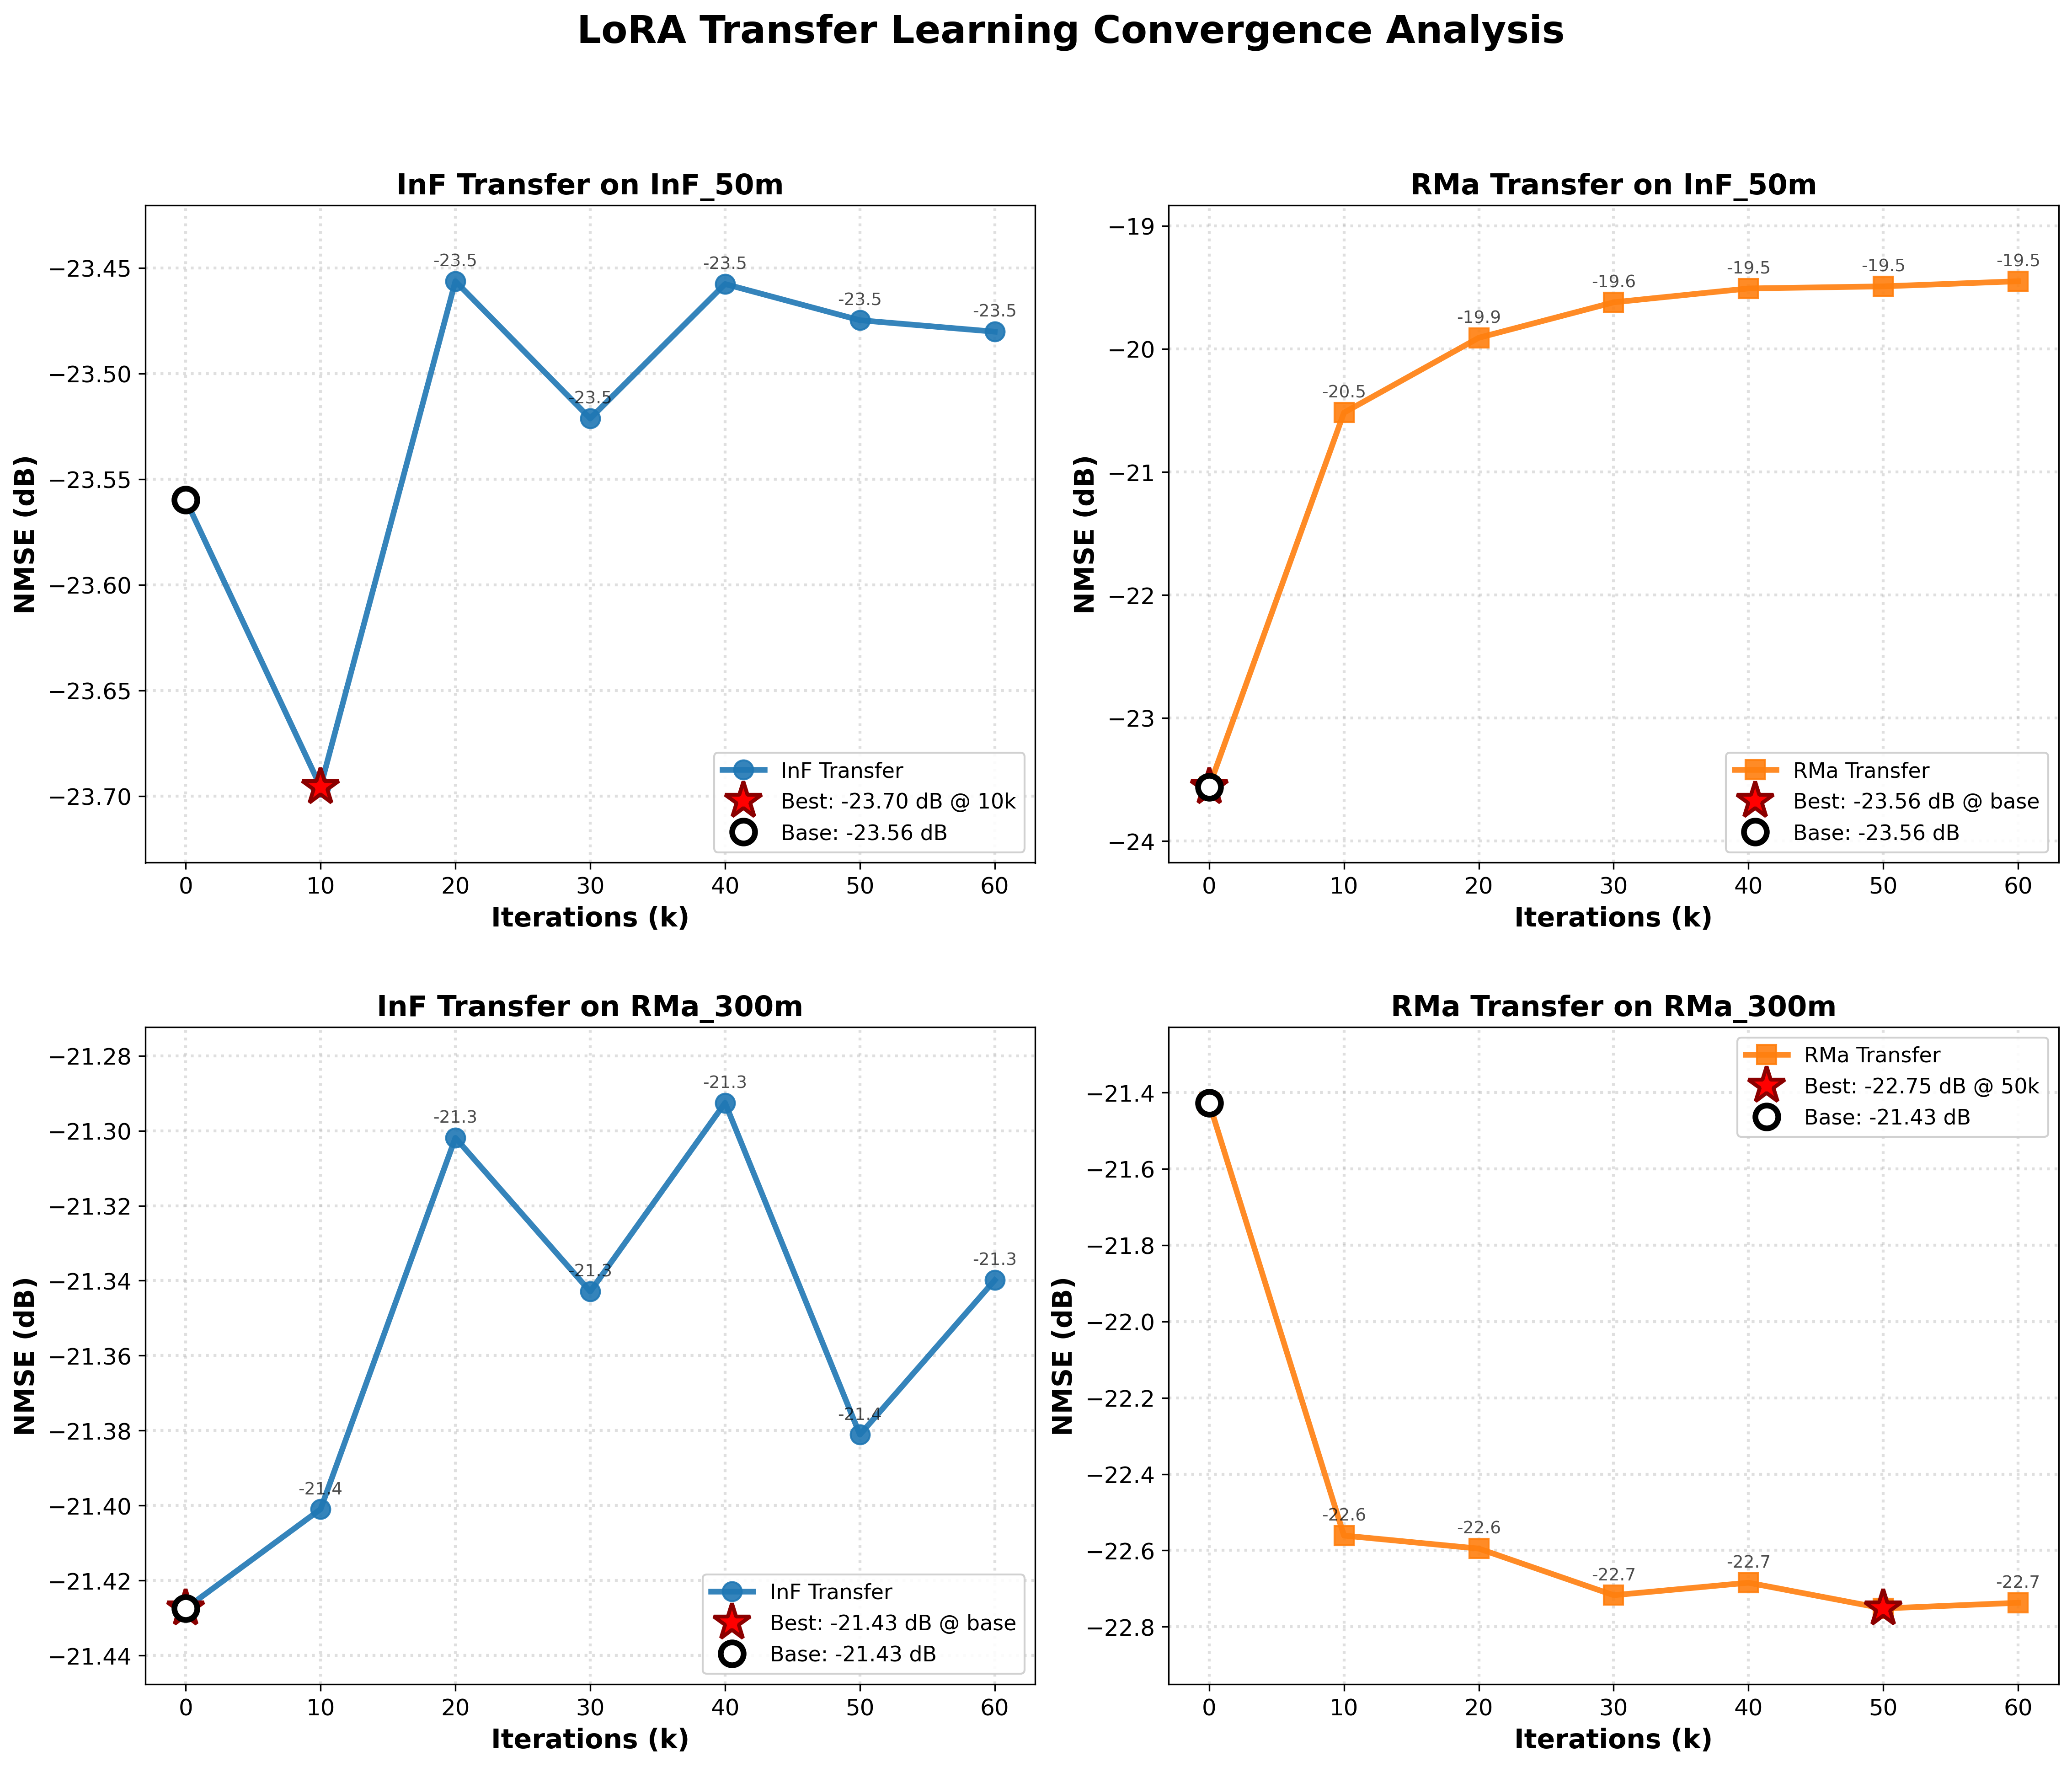
\includegraphics[width=\textwidth]{figures/iteration_convergence_analysis.png}
\caption{Original Convergence Analysis}
\label{fig:convergence_original}
\end{subfigure}
\hfill
\begin{subfigure}[b]{0.48\textwidth}
\centering
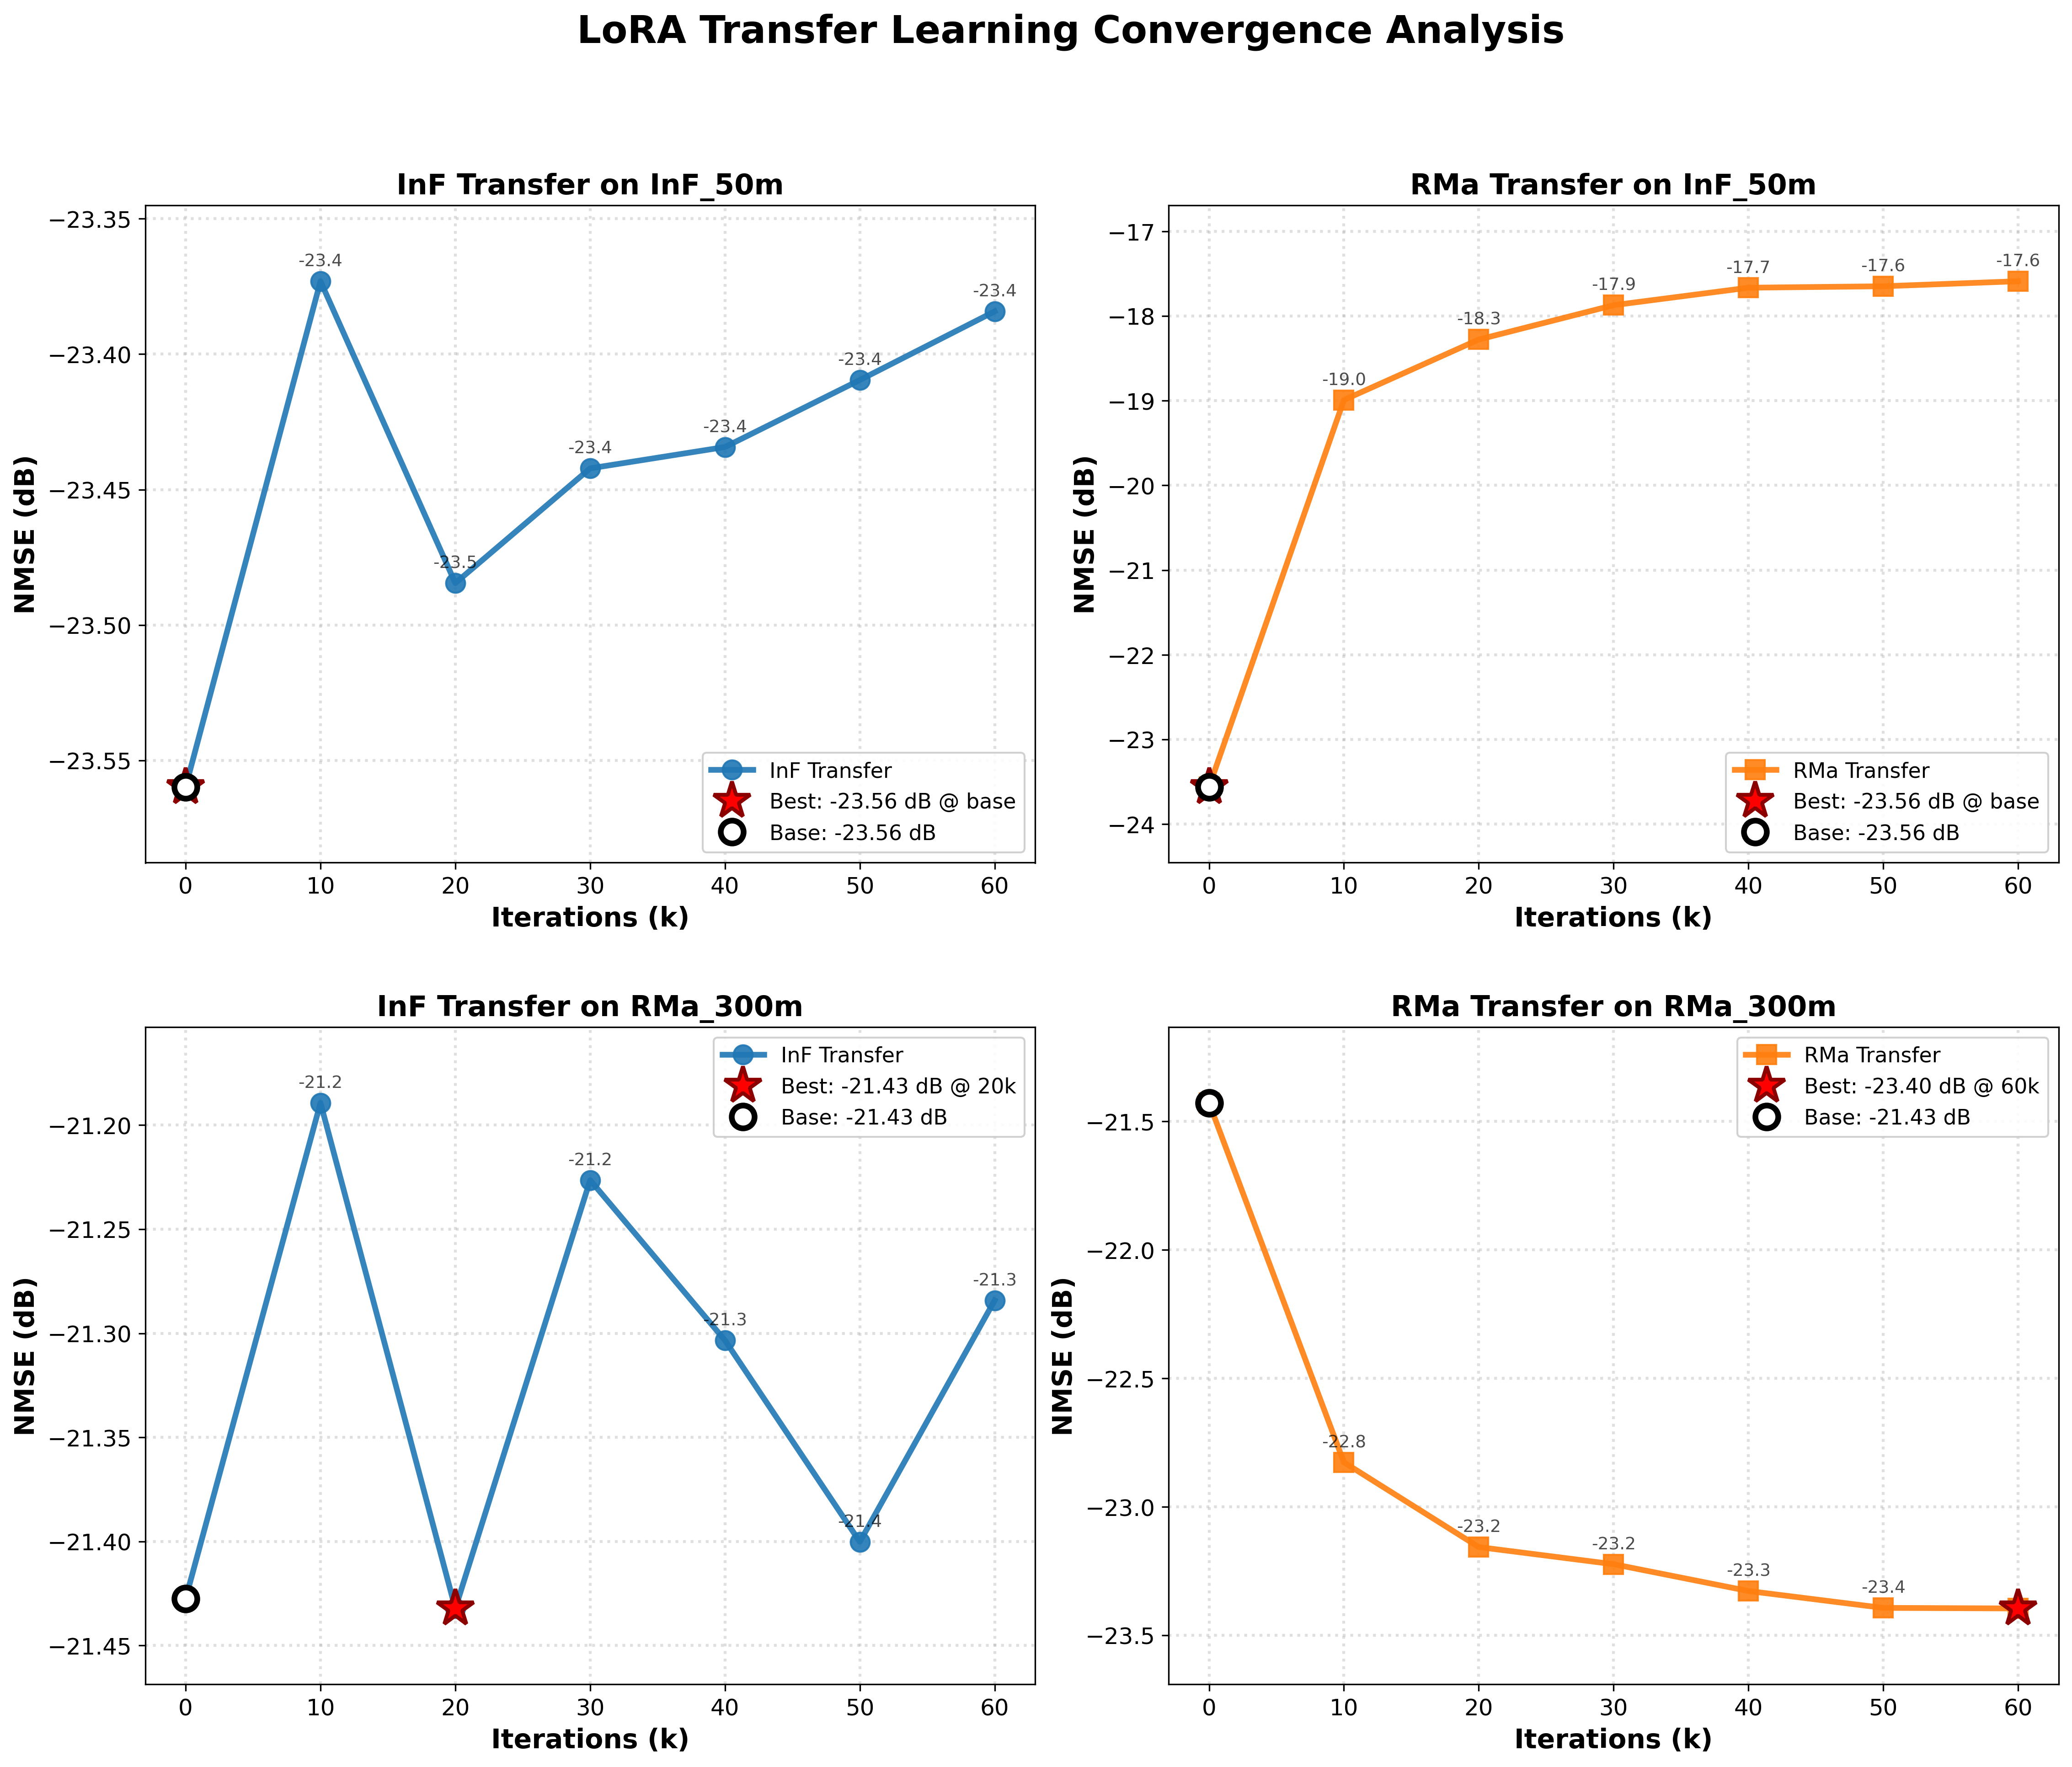
\includegraphics[width=\textwidth]{figures/iteration_convergence_analysis_new_models.png}
\caption{Updated Model Convergence Analysis}
\label{fig:convergence_updated}
\end{subfigure}
\caption{Convergence behavior analysis comparing Adapter and LoRA optimization patterns across different experimental configurations. (a) Initial convergence patterns demonstrating method-specific optimization characteristics across various parameter scales. (b) Enhanced model convergence analysis revealing LoRA's superior optimization efficiency with faster convergence rates and more stable training dynamics, particularly evident in challenging rural environments requiring substantial domain adaptation.}
\label{fig:convergence}
\end{figure}

\subsection{Ablation Studies}

We conducted ablation studies on key hyperparameters using both parameter scales:

\textbf{LoRA Rank Scaling}: Experiments with ranks 4 and 20 demonstrate the parameter-performance trade-off. Rank 4 (26k parameters) provides efficient deployment characteristics, while rank 20 (133k parameters) achieves superior adaptation performance, particularly in rural environments.

\textbf{Target Modules}: Applying LoRA to query, value, and first feed-forward layers consistently yields optimal performance across both parameter scales compared to other module combinations.

\textbf{Adapter Bottleneck Scaling}: Bottleneck dimensions of 10 (20k parameters) and 64 (131k parameters) both show consistent improvement patterns, with the scaled version providing enhanced capacity for environment-specific adaptation while maintaining practical deployment feasibility.

% Cross-domain transfer learning analysis
\subsection{Cross-Domain Transfer Learning}

To evaluate the generalizability of our parameter-efficient methods, we conducted comprehensive cross-domain transfer learning experiments across four environment pairs: Urban$\leftrightarrow$Rural and Indoor$\leftrightarrow$Outdoor. These experiments demonstrate the practical utility of LoRA for multi-environment wireless deployments.

\subsubsection{Cross-Domain Experimental Setup}
We configured four distinct cross-domain scenarios:
\begin{itemize}
\item \textbf{Urban $\rightarrow$ Rural}: UMa+UMi (source) $\rightarrow$ RMa (target)
\item \textbf{Rural $\rightarrow$ Urban}: RMa (source) $\rightarrow$ UMa+UMi (target)  
\item \textbf{Indoor $\rightarrow$ Outdoor}: InH+InF (source) $\rightarrow$ UMa+UMi+RMa (target)
\item \textbf{Outdoor $\rightarrow$ Indoor}: UMa+UMi+RMa (source) $\rightarrow$ InH+InF (target)
\end{itemize}

Each experiment follows the same transfer learning protocol: base model training on source environments followed by LoRA fine-tuning on limited target data (5k-50k iterations).

\begin{figure}[t]
\centering
\includegraphics[width=0.48\textwidth]{figures/cross_domain_performance_clean.pdf}
\caption{Cross-domain transfer learning performance evaluation across four representative environment pairs demonstrating LoRA's adaptability. The results reveal significant performance variations ranging from 1.3 dB (Indoor→Outdoor) to 12.4 dB (Rural→Urban) improvements, highlighting the asymmetric nature of knowledge transfer between different wireless propagation environments and the method's effectiveness in bridging domain gaps.}
\label{fig:cross_domain}
\end{figure}

\subsubsection{Cross-Domain Results Analysis}
Figure~5 presents the cross-domain transfer learning results. Key observations include:

\textbf{Consistent Improvement}: LoRA achieves significant performance gains across most environment pairs, with improvements ranging from 1.3 dB (Indoor$\rightarrow$Outdoor) to 12.4 dB (Rural$\rightarrow$Urban scenario).

\textbf{Domain Gap Impact}: The Urban$\rightarrow$Rural transfer shows moderate improvement (4.1 dB) while Rural$\rightarrow$Urban shows substantial gains (12.4 dB), indicating asymmetric transfer effectiveness. Indoor$\rightarrow$Outdoor shows modest improvement (1.3 dB), while Outdoor$\rightarrow$Indoor shows minimal change (0.4 dB degradation), suggesting the base model already captures indoor characteristics well.

\textbf{Parameter Efficiency}: All cross-domain adaptations use the same LoRA configuration (26.6k parameters, 0.27\% overhead), demonstrating consistent efficiency across diverse scenarios.

\textbf{Asymmetric Transfer Patterns}: Transfer learning effectiveness shows strong directional dependence, with Rural$\rightarrow$Urban (12.4 dB) significantly outperforming Urban$\rightarrow$Rural (4.1 dB), and Indoor$\rightarrow$Outdoor (1.3 dB) showing limited gains compared to Outdoor$\rightarrow$Indoor (-0.4 dB).

These results validate LoRA's effectiveness for practical multi-environment deployments where network operators need rapid model adaptation across heterogeneous wireless scenarios.

\section{Industry Deployment Considerations}

\subsection{Real-time Requirements}

For practical deployment, inference latency is critical. LoRA's ability to merge with base weights during inference eliminates runtime overhead, making it suitable for real-time applications.

\subsection{Edge Device Constraints}

With growing deployment of edge computing in wireless networks, memory efficiency becomes crucial. LoRA's 79\% parameter reduction enables deployment on resource-constrained edge devices.

\subsection{Update Frequency}

In dynamic wireless environments, models require periodic updates. LoRA's fast convergence (33\% fewer iterations) reduces update time and computational cost.

\section{Conclusion}

This paper presented the first comprehensive comparison of Adapter and LoRA methods for parameter-efficient channel estimation, including rigorous parameter scaling analysis to ensure fair comparison. Our experimental results demonstrate that LoRA achieves superior performance across multiple parameter scales and shows distinct advantages in challenging rural environments.

Key findings include:
\begin{itemize}
\item Fair parameter comparison: Nearly identical parameter budgets (131k vs 133k) enable unbiased method evaluation
\item Environment-specific adaptation: LoRA achieves 48\% better adaptation in rural scenarios (-1.97 dB vs -1.33 dB)
\item Base model saturation effect: Minimal InF improvement (+0.08 dB) indicates comprehensive multi-environment training captures indoor characteristics
\item Parameter scaling benefits: Both methods improve with increased capacity (1.2-2.1 dB gains), validating industry-standard 1-3\% parameter usage
\item Convergence efficiency: LoRA demonstrates flexible convergence patterns (20k for InF, 60k for RMa) compared to consistent Adapter requirements
\end{itemize}

While our evaluation utilizes standardized 3GPP channel models for systematic comparison, real-world deployment would require fine-tuning with actual channel measurements specific to the target environment. Nevertheless, these results provide valuable baseline expectations and demonstrate that LoRA's parameter efficiency significantly reduces the data collection burden for adaptation.

\textbf{Future Work}: Our research opens several promising directions for advancing parameter-efficient channel estimation:

\textbf{Digital Twin Integration}: Validation using digital twin frameworks that replicate real-world wireless environments with dynamic channel conditions, interference patterns, and time-varying propagation characteristics will bridge the simulation-reality gap.

\textbf{Advanced Simulation Platforms}: Extension to Sionna-based ray-tracing simulations will enable more accurate modeling of complex propagation scenarios including urban canyon effects, indoor-outdoor transitions, and realistic antenna patterns with sub-6GHz and mmWave frequencies.

\textbf{MIMO Extension}: Adaptation of parameter-efficient methods to MIMO channel estimation will address spatial correlation, multi-stream interference, and beamforming integration in massive MIMO systems, crucial for 6G deployment scenarios.

\textbf{6G Technologies Integration}: Extension to emerging 6G technologies including reconfigurable intelligent surfaces (RIS)-assisted channel estimation, terahertz (THz) band communications with unique propagation characteristics, and joint sensing-communication systems will enable next-generation wireless applications.

The parameter efficiency demonstrated here is particularly relevant as operators face the challenge of deploying models across heterogeneous network environments with limited computational resources.

\section*{Acknowledgment}

The authors would like to thank the Electronics and Telecommunications Research Institute (ETRI) for their valuable support and guidance. This work was also supported by the BK21 FOUR program through the National Research Foundation of Korea (NRF) funded by the Ministry of Education.

\bibliographystyle{IEEEtran}
\bibliography{references}

\end{document}